\documentclass[11pt]{scrartcl}
\usepackage[utf8]{inputenc}
\usepackage{amsmath, amsfonts,amssymb}
\usepackage{graphicx}
\usepackage{xcolor}
\usepackage[format=hang,font=small,labelfont=bf]{caption}
% \usepackage{algorithmicx}
% \usepackage{algorithm}
% \usepackage[noend]{algpseudocode}
% \usepackage{booktabs}
% \usepackage{mathtools}
% \usepackage{float}
% \usepackage{floatpag}
% \usepackage{comment}
% \usepackage{cases}
% \usepackage{mathtools}

%%%%%% PREAMBLE

\newtheorem{theorem}{Theorem}
\newtheorem{lemma}{Lemma}
\DeclareMathOperator*{\argmax}{arg\,max}
\DeclareMathOperator*{\argmin}{arg\,min}
\DeclareMathOperator*{\unif}{Unif}
\DeclareMathOperator*{\bin}{Bin}

\newcommand{\todo}[1]{\textcolor{red}{TODO:
    #1}\PackageWarning{TODO:}{#1!}}

\newcommand{\N}{\mathbb{N}} % naturals
\newcommand{\Q}{\mathbb{Q}} % rationals
\newcommand{\Z}{\mathbb{Z}} % integers
\newcommand{\R}{\mathbb{R}} % reals
\newcommand{\ep}{\varepsilon}
\newcommand{\expect}[1]{\operatorname{\textnormal{\textbf{E}}}\left[#1\right]}
\newcommand{\prob}[1]{\operatorname{\textnormal{Pr}}\left(#1\right)}

%%%%%% TITLE

\title{Ecological Genomics: Homework \#3}
\author{Brendan Case\\
\footnotesize{\texttt{https://github.com/brendandaisy/ecological-genomics}}}
\date{10 April 2020}

\begin{document}
\maketitle

\section{Background}
\label{sec:background}

The copepod \textit{Acartia tonsa} inhabits estuaries and coastal
waters across the world, tolerating a number of different
environmental stressors. Often appearing with high abundance, these
resilient zooplankton are an important base to food chains and other
ecosystem functions.
%
In the turbulent times of the anthropocene, understanding the
mechanisms facilitating rapid adaptation is paramount. While it is
known that DNA methylation has a potential role in adaptation, the
relative importance of epigenenic factors in stress response is still
largely unexplored \cite{Boyko2010, Flores2013}. Here we look for
differences in CpG methylation levels between experimental
\textit{A. tonsa} populations under heat and/or CO$_2$ stress.

\section{Bioinformatics Pipeline}
\label{sec:bioinf-pipel}

Wild \textit{A. tonsa} samples were raised in common garden conditions
for 3 generations prior to being split into the 4 treatments $\times$
4 replicates with $\sim 4,000$ individuals each. Treatments were
control (AA), CO$_2$ stress (AH), heat stress (HA), and combined
stress (HH). Individuals were then let to evolve in these conditions,
and sequencing was performed at both the F0 and F25 generations. For
this study, in the F0 generation we chose only to use the AA
populations. In order to quantify methylation frequencies in each
group, we used reduced representation bisulfite sequencing. Read
quality before and after trimming was performed with
\texttt{fastqc}. In addition, samples were spiked with unmethylated
\textit{E. coli} DNA to test bisulfite conversion
efficiency. Alignment was done using \texttt{bismark} with a reference
\textit{A. tonsa} genome. Samples with expectionally low or high (read
depth $<20$, or $>97.5$th percentile) coverage were removed, then
percent methylation was calculated for each site. Then, differential
methylation was evaluated between the F0 and F25 groups, along with
the AA\_F25 and AH\_F25 groups using hierarchical clustering and
$\chi^2$ tests using the \texttt{methylKit} package in R
\cite{Akalin2012}. Finally, sites with significant methylation
differences between the AA\_F25 and AH\_F25 groups were annotated
using \texttt{bedtools}.

\section{Results}
\label{sec:results}

After filtering, coverage was between 30 and 70 in all groups, with
the highest coverage occurring in the F0 samples. Average percent
methylation was highest in the AA\_F0 group (\%41.3), and lowest in
the AH\_F25 group (\%38.0). Hierarchical clustering between replicates
revealed large-scale differences in methylation percentages between
the F0 generation and the F25 populations (Fig. \ref{fig:1},
left). Further, 3 out of the 4 AA\_F25 and HH\_F25 groups were
distinct from each other, falling into separate ``second level''
branches in the clustering tree. Between the AA\_F25 and AH\_F25
groups, the $\chi^2$ test found 30 sites which were differently
methylated (6 hyper-methylated in AH\_F25, 24 hypo-methylated). Of
these sites, 3 were functionally enriched, with matching GO terms for
DNA integration, dUTP catabolic processes, and various aspects of
endonuclease activity. The two of these SNPs associated with
endonuclease activity were hypo-methylated with similar methylation
levels, while the dUTP-associated SNP was hyper-regulated
(Fig. \ref{fig:1}, right).

\begin{figure}
  \centering
  \begin{minipage}{.45\linewidth}
    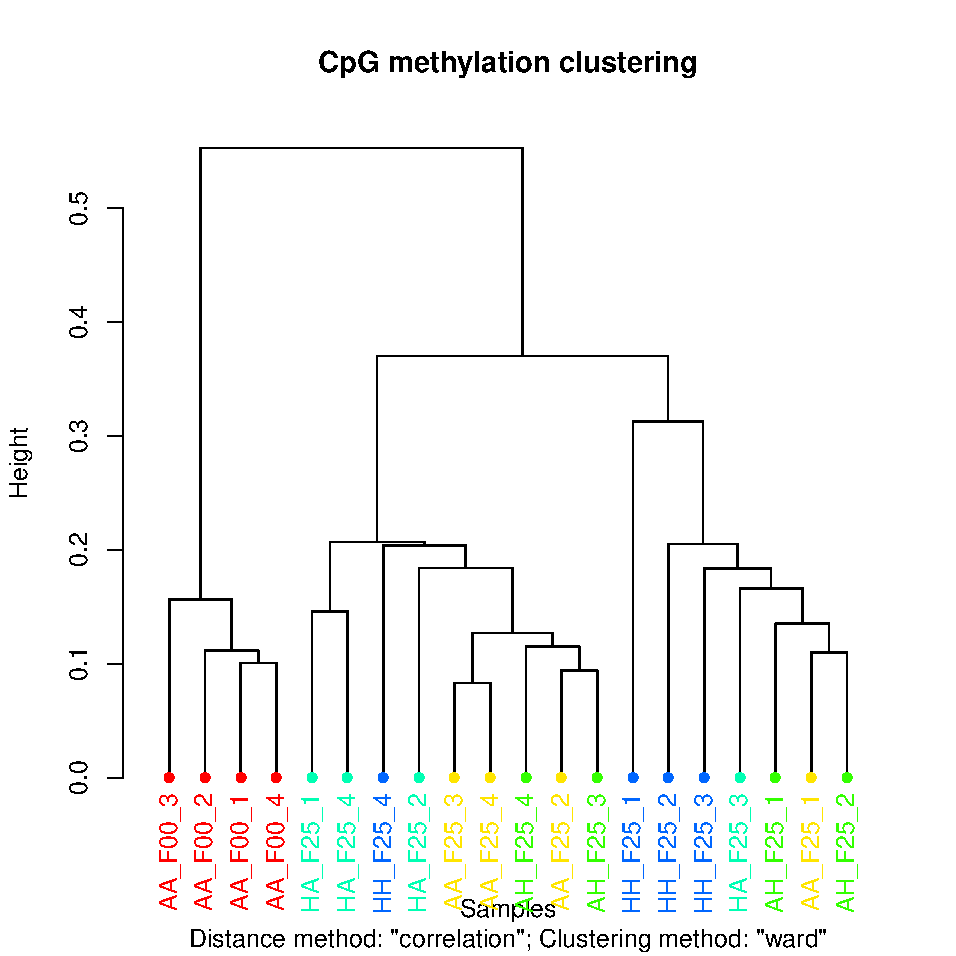
\includegraphics[width=\linewidth]{hclust}
  \end{minipage}
  \begin{minipage}{.45\linewidth}
    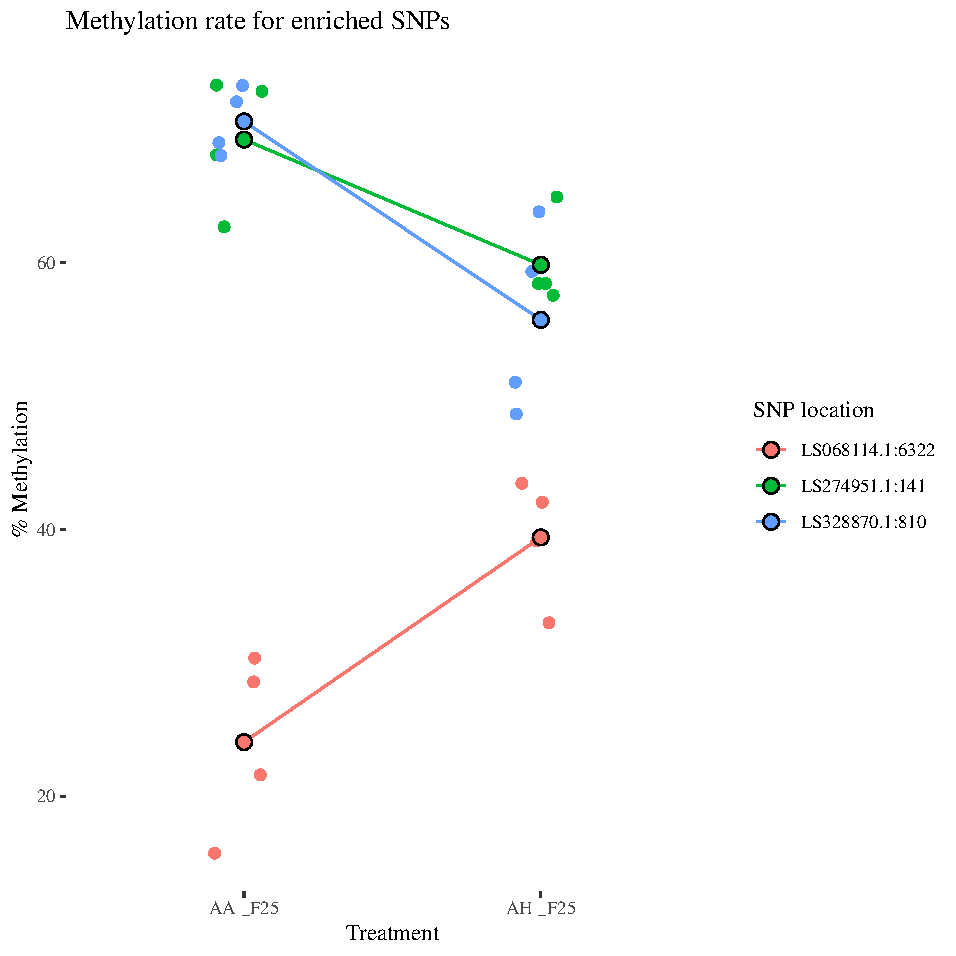
\includegraphics[width=\linewidth]{snp-diff}
  \end{minipage}
  \caption{{\footnotesize Left: hierarchical clustering of methylated percentage in
      all replicate groups. Right: percent methylation in the 3 sites
      which showed significant differences between the AA\_F25 and
      AH\_F25 groups, and were functionally enriched. Larger points
      connected by lines show means for each group, while lines show
      degree of hyper/hypo-methylation.}}
  \label{fig:1}
\end{figure}

\section{Conclusion}
\label{sec:conclusion}

Our results show CpG methylation is present in \textit{A. tonsa} under
a variety of environmental conditions. The largest differences in
methylation was found between F0 and F25 individuals, with methylation
decreasing in the F25 population. While this could suggest a decrease
in methylation associated with adaptation to stress \cite{Cao2011}, it
is also could be an artifact of our sequencing and/or mapping
methods. We also found significantly different methylation levels in
several locations between AA\_F25 and AH\_F25 individuals, which shows
an association between methylation and prolonged CO$_2$ exposure. Two
of these sites were associated with endonuclease activity. While it
was outside the scope of these study to investigate functional roles
in these genes and their association to methylation in response to
stress, this is an avenue for future work.

\newpage

\bibliographystyle{abbrv}
\bibliography{C:/Users/brendandaisy/Documents/citations/ecological-genomics, ../bibextra}

\end{document}

%%% Local Variables:
%%% mode: latex
%%% TeX-master: t
%%% End:
